\documentclass{beamer}

\usepackage[T2A]{fontenc}
\usepackage[utf8]{inputenc}
\usepackage[russian]{babel}

\usepackage{graphicx}
\usepackage{amsmath}
\usepackage{listings}
\usepackage[center]{caption}

\usetheme{Madrid}
\usecolortheme{seagull}

\lstset{
	commentstyle=\color{green!80},
    keywordstyle=\color{blue},
    stringstyle=\color{red},
	tabsize=4,
	basicstyle=\ttfamily
}

\graphicspath{ {./images/} }

\begin{document}

\title[Теория графов] {Теория графов и её приложения}
\subtitle{Отчёт по проектному заданию}
\author[Козырев С., Куклин Д.] {Козырев~С.~А., Куклин~Д.~В.}
\institute[СПбГУ]
{
  Факультет прикладной математики --- процессов управления\\
  Санкт-Петербургский государственный университет
}
\date[\today]{\today}
\logo{
\includegraphics[height=1.5cm]{images/uni-logo.png}}

\frame{\titlepage}

\section{Постановка задачи и методы решения}

\begin{frame}
\frametitle{Постановка задачи}
Требовалось:
\begin{enumerate}
\pause
\item построить граф дорог Российского города,
\pause
\item оценить удобство размещения зданий,
\pause
\item спланировать размещение зданий.
\end{enumerate}
\end{frame}

\begin{frame}
\frametitle{Что мы выбрали}
\begin{enumerate}
\item C++ \pause, так как
	\begin{itemize}
	\item большинство проектов написаны либо на C, либо на C++,
	\pause	
	\item среди остальных C++ является наиболее быстрым,
	\pause
	\item Python простой,
	\end{itemize}
\pause
\item \textit{libosmium},
\pause
\item Нижний Новгород.
\end{enumerate}
\end{frame}

\subsection{Построение графа дорог}

\begin{frame}
\frametitle{OSM Specification}
Спецификация \textit{OSM} определяет следующие структуры данных:
\begin{itemize}
\item \textit{Node} (узел),
\item \textit{Way} (путь),
\item \textit{Relation} (отношение).
\end{itemize}
\end{frame}

\begin{frame}
\frametitle{Извлечение карты}
\begin{figure}[ht]
	\centering	
	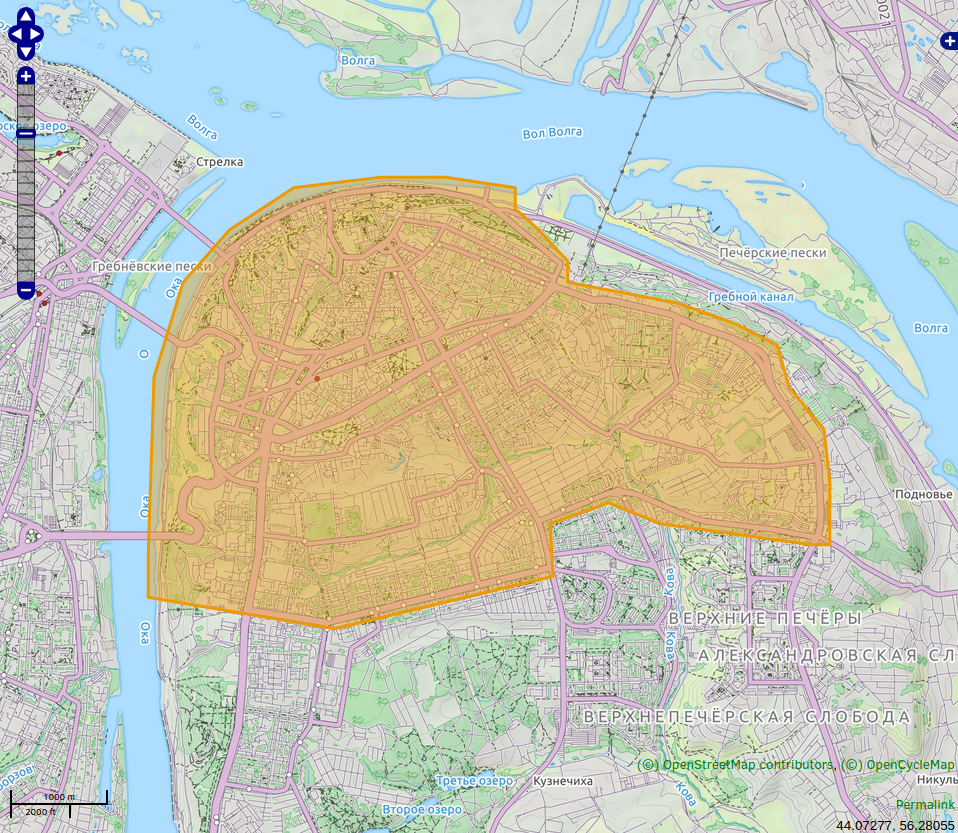
\includegraphics[width=0.4\textwidth]{images/bbbike.png}
	\caption{Карта центра Нижнего Новгорода}
	\label{fig:bbbike}
	\end{figure}
\end{frame}

\begin{frame}[fragile]
\frametitle{Добавление путей}
\lstinputlisting[language=C++]{snippets/mark.cpp}
\end{frame}

\begin{frame}[fragile]
\frametitle{Добавление путей}
\lstinputlisting[language=C++]{snippets/fill.cpp}
\end{frame}

\begin{frame}
\frametitle{Расстояние между узлами}
Расстояние между двумя узлами можно вычислить, используя формулу гаверсинуса
\begin{gather*}
	\eta(\Theta) = \eta(\varphi_2 - \varphi_1) + \cos(\varphi_1) \cos(\varphi_2) \eta(\lambda_2 - \lambda_1), \\
	d = 2r \arcsin(\sqrt{\eta(\Theta)}),
\end{gather*}
	где $ \Theta $~--- центральный угол, $ \varphi_{1,2} $~--- широты в радианах, $ \lambda_{1,2} $~--- высоты в радианах и $ \eta(\theta) = \sin^2\left(\frac{\theta}{2}\right) $ для произвольного угла $ \theta $.
\end{frame}

\begin{frame}[fragile]
\frametitle{Структура \texttt{Node}}
\lstinputlisting[language=C++]{snippets/node.cpp}
\end{frame}

\begin{frame}[fragile]
\frametitle{Структура \texttt{Graph}}
\lstinputlisting[language=C++]{snippets/graph.cpp}
\end{frame}

\begin{frame}
\frametitle{Структура \texttt{Building}}
Для каждого здания на карте
\begin{enumerate}
\item вычисляем барицентр здания,
\item находим ближайший к зданию узел дороги,
\item в структуре \textit{Building} связываем со зданием найденный узел.
\end{enumerate}
\end{frame}

\begin{frame}[fragile]
\frametitle{Структура \texttt{Building}}
\lstinputlisting[language=C++]{snippets/building.cpp}
\end{frame}

\begin{frame}[fragile]
\frametitle{Структура \texttt{Map}}
\lstinputlisting[language=C++]{snippets/map.cpp}
\end{frame}

\begin{frame}
\frametitle{Проблема производительности}
Очевидно, карта составляется долго.\\
\textit{Libosmium} каждый раз производит чтение карты и заполнение структур.\\
Вопрос итоговой сложности является открытым, но любой желающий может получить на него ответ, изучив исходный код библиотеки.
\end{frame}

\begin{frame}[fragile]
\frametitle{Кэширование}
Мы обошли проблему, применив кэширование к структуре \texttt{Map}.\\
\lstinputlisting[language=C++]{snippets/serialize.cpp}
\end{frame}

\begin{frame}[fragile]
\frametitle{Кэширование}
\lstinputlisting[language=C++]{snippets/deserialize.cpp}
\end{frame}

\subsection{Оценка удобства размещения объектов инфраструктуры}
\begin{frame}
\frametitle{Задача}
Требовалось выбрать $ M $ объектов инфраструктуры и $ N $ жилых зданий и оценить удобство их размещения, используя расстояние как метрику.
\lstinputlisting[language=C++]{snippets/categories.cpp}
\end{frame}
    
\begin{frame}
\frametitle{Выбор ближайшего узла}
Для каждого здания запоминаем ближайший узел.
\lstinputlisting[language=C++]{snippets/closest.cpp}
\end{frame}

\begin{frame}
\frametitle{Алгоритм Дейкстры}
Нами был реализован алгоритм Дейкстры с временной сложностью $ O(n \log n) $.\\
Используя алгоритм, несложно как и определить ближайшие объекты, так и построить дерево кратчайших путей.
\end{frame}

\begin{frame}
\frametitle{Оценка планирования}
\lstinputlisting[language=C++]{snippets/minmax_1.cpp}
\end{frame}

\begin{frame}
\frametitle{Оценка планирования}
\lstinputlisting[language=C++]{snippets/minmax_2.cpp}
\end{frame}

\begin{frame}
	\frametitle{Иерархическая кластеризация}
	\begin{itemize}
		\item вычисляем матрицу расстояний
		\item из каждого дома делаем кластер
		\item дальше добавляем новые кластеры путём объдинения двух ближайших, пока не останется только один класс без предка
	\end{itemize}
\end{frame}

\begin{frame}
	\frametitle{Иерархическая кластеризация}
	\begin{itemize}
		\item вычисляем матрицу расстояний
	\end{itemize}
\end{frame}

\begin{frame}
	\frametitle{Иерархическая кластеризация}
	\begin{itemize}
		\item вычисляем матрицу расстояний
		\item из каждого дома делаем кластер
	\end{itemize}
\end{frame}

\begin{frame}
	\frametitle{Иерархическая кластеризация}
	\begin{itemize}
		\item вычисляем матрицу расстояний
		\item из каждого дома делаем кластер
		\item дальше добавляем новые кластеры путём объдинения двух ближайших, пока не останется только один класс без предка
	\end{itemize}
\end{frame}

\begin{frame}
	\frametitle{Матрица расстояний}
	Матрицу расстояний вычисляем путём запуска алгоритма Дейкстры из каждой вершины.
\end{frame}

\begin{frame}
	\frametitle{Пример}
	Дано 15 домов, будем разбивать их на кластеры, находить длину деревьев кратчайших путей, и сумму кратчайших путей.

\end{frame}

\begin{frame}
	\frametitle{1 кластер; 32,3 км; 12,8 км}
	\centering
	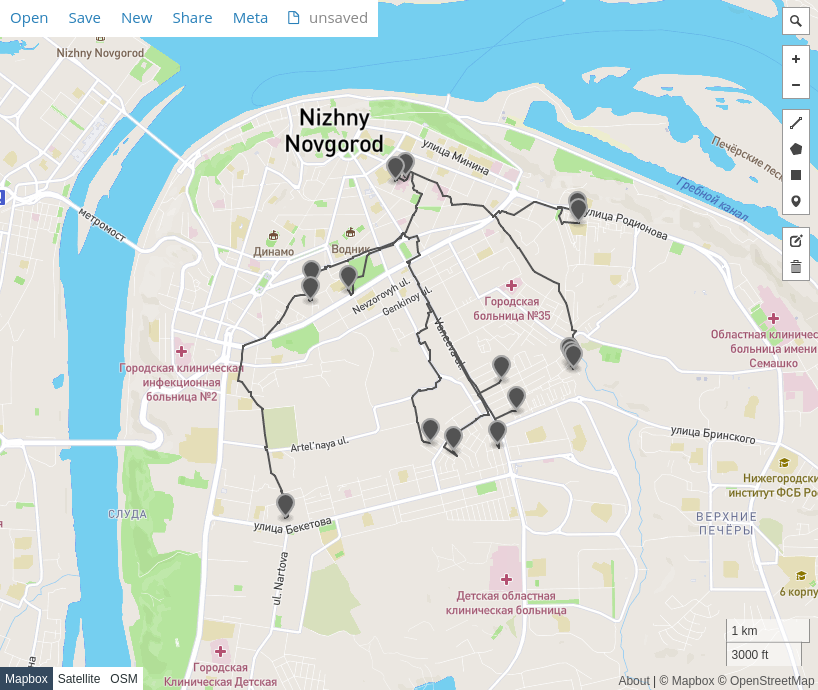
\includegraphics[width=0.65\textwidth]{k1}
\end{frame}

\begin{frame}
	\frametitle{2 кластера; 13,2 км; 8,2 км}
	\centering
	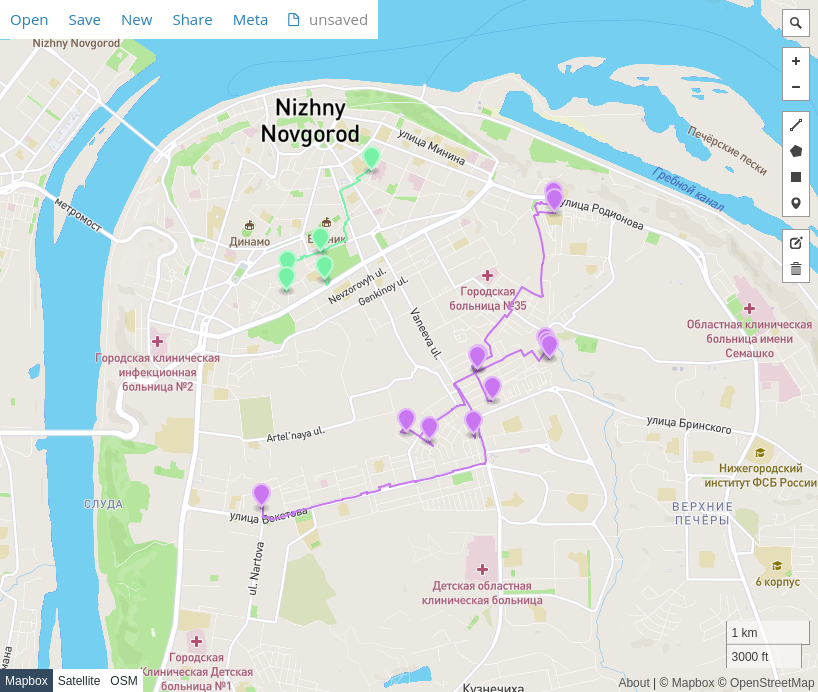
\includegraphics[width=0.65\textwidth]{k2}
\end{frame}

\begin{frame}
	\frametitle{3 кластера; 11,3 км; 6,3 км}
	\centering
	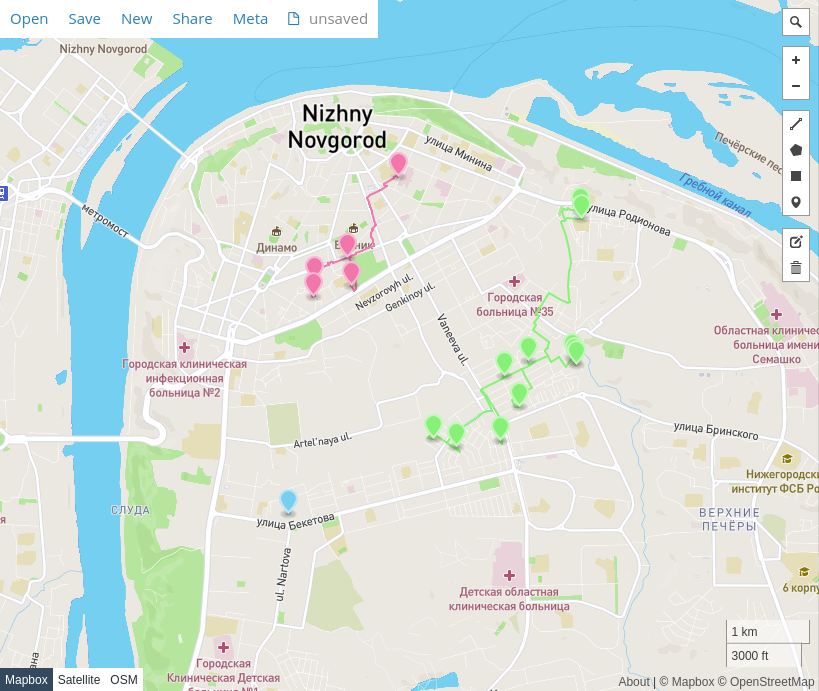
\includegraphics[width=0.65\textwidth]{k3}
\end{frame}

\begin{frame}
	\frametitle{5 кластеров; 4,6 км; 3,9 км}
	\centering
	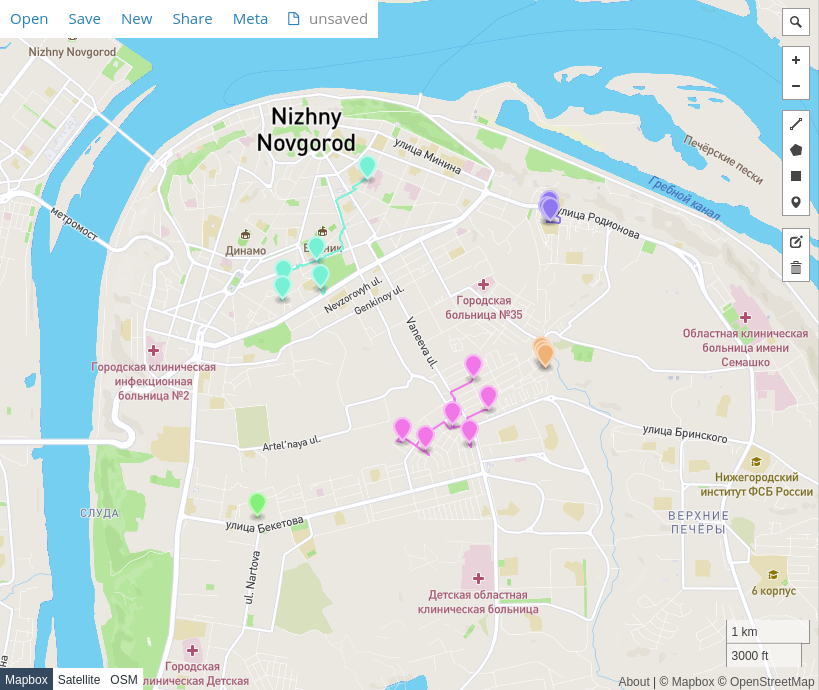
\includegraphics[width=0.65\textwidth]{k5}
\end{frame}

\begin{frame}
	\frametitle{Дендрограмма}
	\centering
	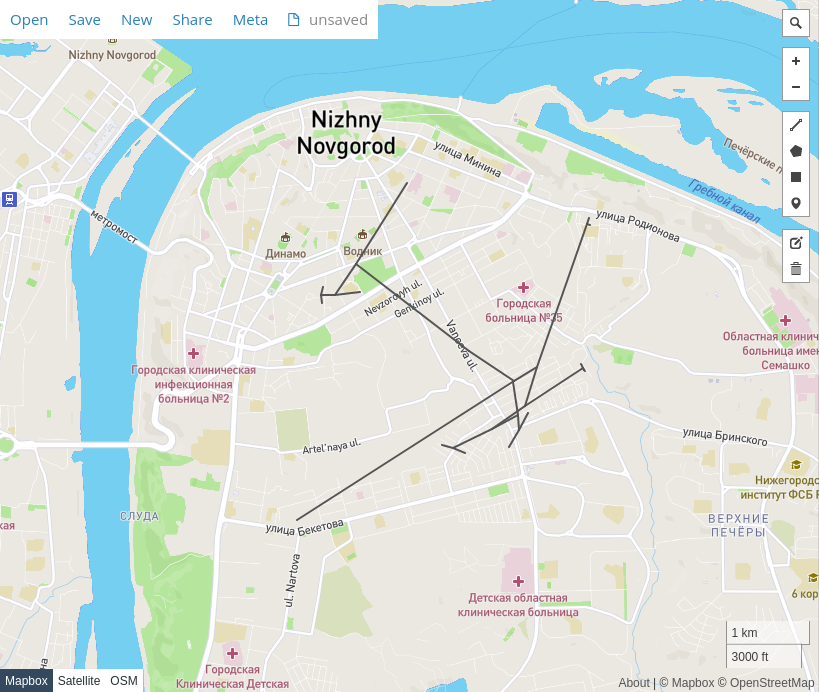
\includegraphics[width=0.65\textwidth]{dendrogram}
\end{frame}

\end{document}